\documentclass[11pt,]{article}
\usepackage{lmodern}
\usepackage{amssymb,amsmath}
\usepackage{ifxetex,ifluatex}
\usepackage{fixltx2e} % provides \textsubscript
\ifnum 0\ifxetex 1\fi\ifluatex 1\fi=0 % if pdftex
  \usepackage[T1]{fontenc}
  \usepackage[utf8]{inputenc}
\else % if luatex or xelatex
  \ifxetex
    \usepackage{mathspec}
  \else
    \usepackage{fontspec}
  \fi
  \defaultfontfeatures{Ligatures=TeX,Scale=MatchLowercase}
\fi
% use upquote if available, for straight quotes in verbatim environments
\IfFileExists{upquote.sty}{\usepackage{upquote}}{}
% use microtype if available
\IfFileExists{microtype.sty}{%
\usepackage{microtype}
\UseMicrotypeSet[protrusion]{basicmath} % disable protrusion for tt fonts
}{}
\usepackage[margin=1in]{geometry}
\usepackage{hyperref}
\PassOptionsToPackage{usenames,dvipsnames}{color} % color is loaded by hyperref
\hypersetup{unicode=true,
            colorlinks=true,
            linkcolor=black,
            citecolor=Blue,
            urlcolor=black,
            breaklinks=true}
\urlstyle{same}  % don't use monospace font for urls
\usepackage{graphicx,grffile}
\makeatletter
\def\maxwidth{\ifdim\Gin@nat@width>\linewidth\linewidth\else\Gin@nat@width\fi}
\def\maxheight{\ifdim\Gin@nat@height>\textheight\textheight\else\Gin@nat@height\fi}
\makeatother
% Scale images if necessary, so that they will not overflow the page
% margins by default, and it is still possible to overwrite the defaults
% using explicit options in \includegraphics[width, height, ...]{}
\setkeys{Gin}{width=\maxwidth,height=\maxheight,keepaspectratio}
\IfFileExists{parskip.sty}{%
\usepackage{parskip}
}{% else
\setlength{\parindent}{0pt}
\setlength{\parskip}{6pt plus 2pt minus 1pt}
}
\setlength{\emergencystretch}{3em}  % prevent overfull lines
\providecommand{\tightlist}{%
  \setlength{\itemsep}{0pt}\setlength{\parskip}{0pt}}
\setcounter{secnumdepth}{0}
% Redefines (sub)paragraphs to behave more like sections
\ifx\paragraph\undefined\else
\let\oldparagraph\paragraph
\renewcommand{\paragraph}[1]{\oldparagraph{#1}\mbox{}}
\fi
\ifx\subparagraph\undefined\else
\let\oldsubparagraph\subparagraph
\renewcommand{\subparagraph}[1]{\oldsubparagraph{#1}\mbox{}}
\fi

%%% Use protect on footnotes to avoid problems with footnotes in titles
\let\rmarkdownfootnote\footnote%
\def\footnote{\protect\rmarkdownfootnote}

%%% Change title format to be more compact
\usepackage{titling}

% Create subtitle command for use in maketitle
\newcommand{\subtitle}[1]{
  \posttitle{
    \begin{center}\large#1\end{center}
    }
}

\setlength{\droptitle}{-2em}
  \title{}
  \pretitle{\vspace{\droptitle}}
  \posttitle{}
  \author{}
  \preauthor{}\postauthor{}
  \date{}
  \predate{}\postdate{}

\usepackage{amsmath,amssymb}
\usepackage{cite}
\usepackage{nameref,hyperref}
\usepackage[left]{lineno}
\usepackage[font=small,labelfont=bf]{caption}
\usepackage{mathptmx}
\usepackage{longtable,booktabs}

\begin{document}

\raggedright\vspace*{0.2in}

\begin{centering}

{\Large
\textbf\newline{Linking early warning signals to the temporal epidemiology of measles in Nigerien cities} 
}

\vspace{2em}

Andrew T. Tredennick\textsuperscript{1,2}\footnote{Corresponding author: atredenn@gmail.com},
Pejman Rohani\textsuperscript{1,2},
Eamon O'Dea\textsuperscript{1,2},
\& John M. Drake\textsuperscript{1,2}
\\
\bigskip
\textsuperscript{1} \small\emph{Odum School of Ecology, University of Georgia, Athens, GA, USA} \\
\textsuperscript{2} \small\emph{Center for the Ecology of Infectious Diseases, University of Georgia, Athens, GA, USA}

\end{centering}

\hypertarget{abstract}{%
\section{Abstract}\label{abstract}}

Forecasting the trajectory of infectious disease outbreaks over time is
a fundamental challenge facing society.

\linenumbers

\hypertarget{introduction}{%
\section{Introduction}\label{introduction}}

Theory shows that epidemic transitions can be anticipated by trends in
the statistical properties of disease time series (AERO papers). The
existence of statistical trends in the data that precede critical
transitions, so-called `early warning signals' (EWS), imply that we may
be able to anticipate disease emergence and outbreaks. The end goal is a
model-independent detection system, where statistical properties of
disease surveilence data can trigger warnings of impending outbreaks
without the need to fit mechanistic models of disease transmission (Han
and Drake 2017).

However, there is currently a gap between the theoretical work, which
has relied on knowing the underlying disease dynamics, and the eventual
goal of applying EWS in real-world situations where the underlying
disease dynamics may be unknown. Theoretical development of EWS has
focused on anticipating when the population becomes supercritical, when
\(\mathcal{R}_0 > 1\), after which an outbreak is inevitable, perhaps
with some bifurcation delay (Dibble et al.~2016). Knowing the value of
\(\mathcal{R}_0\) through time makes it possible to test the accuracy of
EWS that are estimated from state variables alone. Empirical application
of EWS does not require knowing the value of \(\mathcal{R}_0\) through
time, meaning that ``tests'' require making assumptions about when
critical transitions occur. Whether EWS track and/or anticipate
underlying dynamics of real disease time series remains unknown, and is
a critical knowledge gap that must be filled before EWS can confidently
be deployed.

To fill this gap we will fit a mechanistic model to incidence data of
measles in Niger to estimate the temporal epidemiology of the disease,
yielding the very same parameters that are known in data-free modeling
studies. In particular, we are interested in the correlation between EWS
and the time-varying repreoductive ratio, known as the effective
reprodutive ratio \(\left(\mathcal{R}_E\right)\). If EWS and
\(\mathcal{R}_E\) are significantly and positively correlated, then we
have empirical evidence that EWS are applicable in real-world settings.
If EWS and \(\mathcal{R}_E\) are negatively correlated or not
significantly posivitely correlated, then we have evidence that EWS may
not be applicable in certain settings.

\hypertarget{materials-and-methods}{%
\section{Materials and Methods}\label{materials-and-methods}}

\hypertarget{data}{%
\subsection{Data}\label{data}}

We used weekly measles case report data from four Nigerien cities,
collected over an 11 year period (1995-2005) (Figure \ref{fig:data}).
These data are ideal for stress testing EWS because each city has
different population sizes, has different dynamics in terms of size of
outbreaks and length of inter-epidemic periods, and each time series has
different amounts of ``noise'' (though, the difference in variability is
probably just reflective of population size differences). The data come
from {[}\emph{somewhere/someone}{]}, and used here with permission from
{[}\emph{somewhere/someone}{]}.

\begin{figure}[!ht]
\centering
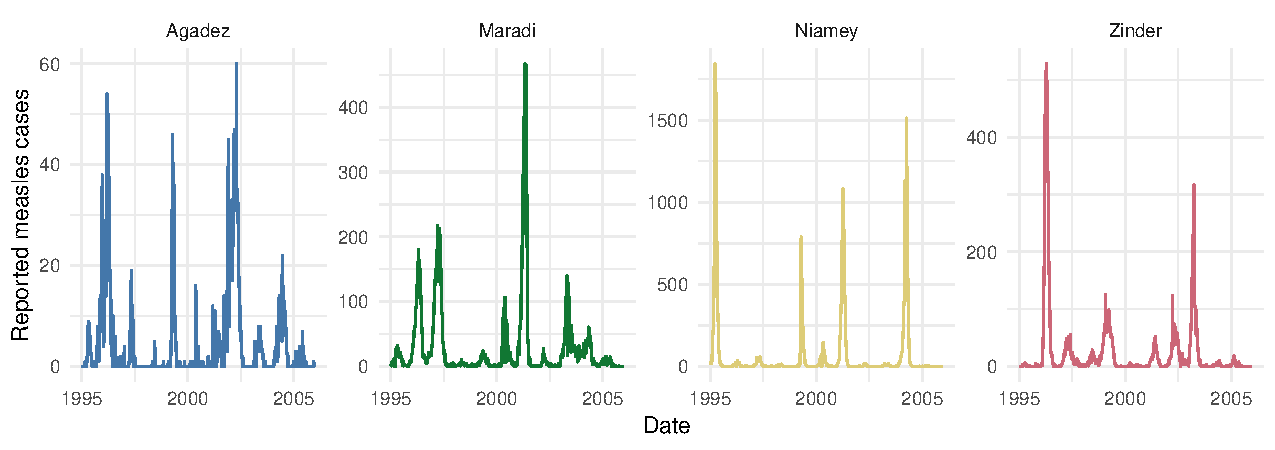
\includegraphics[width=\textwidth]{../figures/data-timeseries.pdf}
\caption{Time series of weekly measles case reports from four cities in Niger.}
\label{fig:data}
\end{figure}

\hypertarget{stochastic-si-model}{%
\subsection{\texorpdfstring{Stochastic \emph{SI}
model}{Stochastic SI model}}\label{stochastic-si-model}}

The model is a continuous time \emph{SI} model with limited demography,
specified as a set of stochastic differential equations:

\begin{align}
dS &= \mu_t N_t dt - \lambda_t S_t dt + dU_t \\
dI &= \psi_t dt + \lambda_t S_t dt - \gamma I_t dt + dV_t
\end{align}

\noindent{}where \(\mu_t\) is birth rate at time \emph{t}, \(\gamma\) is
the time-invariant recovery rate, \(\psi_t\) is rate of imported
infections, \(\lambda_t\) is the time-varying force of infectionm, and
\(U_t\) and \(V_t\) are noise terms. We do not include a death process
in the model because we expect death rates from the susceptible and
infectious classes to be minimal relative to births and we are not
interested in the recovered class since we know total population size.
Excluding deaths means we can avoid making further assumptions about
demographic rates -- we are already making assumptions about birth rates
(e.g., the rate is the same across cities, but with city-specific
population size). We model stochasticity in births and imported
infections by drawing time-specific values from Poisson distributions.
Transitions in the model are shown in Table \ref{table:model-trans}. We
model \(\lambda_t\) as a function of a seasonal tranmission rate subject
to additional environmental variability through time:

\begin{align}
\lambda_t &= \frac{\beta_t I_t}{N_t}, \\
\beta_t &= \beta \left(1 + \sum^6_{i=1} q_i \xi_{i_{t}} \right) \Gamma_t,
\end{align}

\noindent{}where \(\beta_t\) is the rate of transmission at time
\emph{t}, \(\beta\) is the mean transmission rate, \(\psi\) accounts for
measles infections from external sources that are not part of the local
dynamics, and the term \(\sum^6_{i=1} q_i \xi_{i_{t}}\) is a B-spline to
model seasonality in transmission. The B-spline bases (\(\xi_{i_{t}}\))
are periodic with a 1 year period. The transmission rate (\(\beta_t\))
is also subject to stochastic process noise at each time step,
\(\Gamma_t\), which we model as a gamma-distributed white (temporally
uncorrelated) noise with mean 1 and variance \(\sigma^2\) (Bretó and
Ionides 2011). In this model, the effective reproductive ratio at time
\emph{t} is: \(\mathcal{R}_{E(t)} = \beta_t / \gamma\).

We assume observed case reports (\(\textbf{y}\)) are drawn from a
Poisson distribution subject to a constant reporting fraction
(\(\rho\)),

\begin{align}
y_t \sim \text{Poisson} \left( \rho I_t \right).
\end{align}

\textbackslash{}begin\{table\}{[}!ht{]} \centering

\caption{Transitions in the SI model. We show the determinstic transmission rate for clarity, but our model uses the stochastic tranmission rate.}

\textbackslash{}begin\{tabular\}\{lll\} \toprule Transition \&
(\(\Delta S\), \(\Delta I\)) \& Propensity \textbackslash{} \midrule
birth \& \((1, 0)\) \& \(N_t \mu\) \textbackslash{} imported infections
\& \((0, 1)\) \& \(\psi_t\) \textbackslash{} transmission
(deterministic) \& \((-1, 1)\) \& \(SI \beta_t / N_t\) \textbackslash{}
transmission (stochastic) \& \((-k, k)\) \&
\(\frac{S}{k}\sum^k_{j=0} \left(\begin{matrix}k\\j\end{matrix} \right) (-1)^{k-j+1} \tau_{\text{f}}^{-1} \text{ln}(1 + (\beta_tI/N_t)) \tau_{\text{f}} (S-j)\)
\textbackslash{} recovery \& \((0, -1)\) \& \(I\gamma\) \textbackslash{}
\bottomrule \textbackslash{}end\{tabular\} \label{table:model-trans}
\textbackslash{}end\{table\}

\nolinenumbers


\end{document}
